\chapter{Contexte Général et Étude Préalable}
\label{chap:general_context}


\section{Introduction}

\par Ce chapitre introductif présente le cadre général dans lequel ce projet de fin d'études a été réalisé. Il décrit dans un premier temps l'organisme d'accueil ainsi que son contexte professionnel, avant de présenter le cadre général du projet \textbf{RedSys}, en détaillant son activité, son domaine d'expertise ainsi que son environnement de travail.
\par Ensuite, le chapitre présente le contexte du projet \textbf{TuniPark}, une application conçue pour la gestion des places de stationnement. Il souligne les enjeux auxquels sont confrontés les conducteurs lorsqu'ils cherchent une place pour se garer, ainsi que les besoins qui ont conduit à l'élaboration de cette solution. Pour conclure, ce chapitre introduit la proposition de solution, les buts du projet et la méthode suivie pour réussir les diverses étapes de la conception, du développement et de la validation de l'application.


\section{Entreprise d'accueil}

\subsection{Aperçu de RedSys}

\par \textbf{RedSys} est une entreprise tunisienne spécialisée dans les technologies de l'information. Elle intervient principalement dans les domaines des infrastructures informatiques, des réseaux, du cloud et de la cybersécurité. L'entreprise a été créée par des professionnels du secteur avec l'objectif de proposer des solutions informatiques fiables, sécurisées et répondant aux besoins de ses clients.

\begin{figure}[H]
    \centering
    
\includegraphics[width=0.4\textwidth]{img/logo-enterprise.png}
    \caption{Logo de RedSys}
    \label{fig:redsys_logo}
\end{figure}

\par RedSys accompagne les entreprises dans l'intégration, le déploiement et la maintenance de leurs systèmes informatiques. Ses services concernent notamment la mise en place d'infrastructures, l'intégration de solutions réseau, la migration vers le cloud ainsi que la sécurisation des environnements numériques.

\par L'entreprise attache également une grande importance à la qualité de ses services, à la réactivité de ses équipes et à l'évolution des compétences de ses collaborateurs. Cette approche lui permet de proposer des solutions évolutives et de construire des relations durables avec ses clients.


\subsection{Domaines d'activité de RedSys}

\par RedSys accompagne les entreprises dans la conception, le déploiement et la maintenance de solutions informatiques adaptées à leurs besoins. Son activité couvre plusieurs domaines, notamment l'administration des infrastructures informatiques, les réseaux, les services cloud, la cybersécurité ainsi que le développement de solutions numériques.

\par L'entreprise intervient auprès de clients issus de différents secteurs en proposant des services de conseil, d'intégration et de support technique. Elle met également l'accent sur l'innovation et l'utilisation de technologies modernes afin de répondre aux nouveaux besoins liés à la transformation numérique.

\par Grâce à son expertise technique et à son approche orientée qualité, RedSys développe des solutions fiables et évolutives, tout en assurant un accompagnement continu de ses clients.

\subsection{Contexte organisationnel}

\par Dans le cadre de sa stratégie de développement, RedSys encourage la réalisation de projets innovants répondant à des problématiques concrètes. C'est dans cette optique qu'a été proposé le projet \textbf{TuniPark}, une application mobile et une plateforme web destinées à faciliter la gestion et la réservation des places de parking.

\par Ce projet s'inscrit dans une démarche de transformation numérique visant à optimiser l'expérience des utilisateurs en proposant une solution simple, sécurisée et accessible. Il répond également aux besoins des gestionnaires de parkings en leur offrant des outils permettant de suivre et d'administrer efficacement leurs espaces de stationnement.






\section{Cadre général du projet}

\par Le stationnement représente aujourd'hui un défi quotidien pour de nombreux conducteurs, notamment dans les zones urbaines où le nombre de places disponibles est souvent insuffisant. Cette situation engendre une perte de temps, une augmentation de la circulation ainsi qu'une consommation supplémentaire de carburant.

\par En parallèle, de nombreux espaces de stationnement privés restent inoccupés durant une partie de la journée. Ces espaces pourraient être exploités afin de répondre aux besoins des conducteurs tout en offrant une source de revenus complémentaire à leurs propriétaires.

\par Afin de répondre à cette problématique, \textbf{RedSys} a lancé le projet \textbf{TuniPark}. Dans le cadre de ce projet de fin d'études, une application mobile accompagnée d'une interface web d'administration a été conçue et développée afin de faciliter l'accès aux places de stationnement disponibles et de permettre aux propriétaires de proposer leurs espaces.

\section{Problématique}

\par Malgré l'existence de plusieurs solutions de stationnement, celles-ci ne répondent pas toujours aux besoins des conducteurs ni à ceux des propriétaires d'espaces privés. Les conducteurs rencontrent encore des difficultés pour trouver rapidement une place disponible, tandis que de nombreux propriétaires ne disposent pas d'un moyen simple et fiable pour proposer leurs espaces de stationnement.

\par La problématique de ce projet peut ainsi être formulée comme suit :

\begin{quote}
Comment développer une application permettant de faciliter l'accès aux places de stationnement disponibles tout en offrant aux propriétaires un moyen simple et sécurisé de proposer leurs espaces ?
\end{quote}

\section{Étude de l'existant}

\par Plusieurs applications permettent aujourd'hui de rechercher des parkings, de consulter leur localisation et, dans certains cas, d'effectuer un paiement en ligne. La plupart de ces solutions sont principalement orientées vers les parkings publics ou les parkings gérés par des partenaires professionnels.

\par En revanche, elles offrent rarement aux particuliers la possibilité de proposer facilement leurs propres espaces de stationnement. Cette limitation réduit le nombre de places accessibles et ne permet pas d'exploiter pleinement les espaces privés disponibles.

\section{Critique de l'existant}

\par L'étude des solutions existantes met en évidence plusieurs limites. D'une part, l'offre de stationnement reste insuffisante dans certaines zones fortement fréquentées. D'autre part, les propriétaires d'espaces privés disposent de peu d'outils leur permettant de publier et de gérer simplement leurs annonces.

\par Ces limites justifient le développement d'une solution offrant à la fois une expérience simple pour les conducteurs et un moyen efficace pour les propriétaires de mettre leurs espaces de stationnement à disposition.

\section{Solution proposée}

\par Afin de répondre aux limites identifiées lors de l'étude de l'existant, une plateforme nommée \textbf{TuniPark} a été conçue et développée. Elle se compose d'une application mobile destinée aux conducteurs et aux propriétaires de parkings privés, ainsi que d'une interface web dédiée à l'administration de la plateforme.

\begin{figure}[H]
    \centering
    
\includegraphics[width=0.28\textwidth]{img/logo-tunipark.png}
    \caption{Icône de l'application TuniPark}
    \label{fig:tunipark_icon}
\end{figure}

\par L'application mobile offre aux conducteurs la possibilité de localiser des parkings, de consulter leurs informations, d'effectuer un paiement en ligne et de gérer leurs sessions de stationnement. Les propriétaires disposent d'un espace leur permettant de publier leurs parkings, de définir les tarifs, les horaires d'ouverture, la capacité d'accueil et de suivre les revenus générés par leurs espaces.

\par L'interface web est réservée à l'administrateur de la plateforme. Elle permet d'examiner les demandes de création de parkings, de valider ou de refuser les annonces proposées et d'assurer le suivi global du fonctionnement de l'application.

\par D'un point de vue technique, l'application mobile a été développée avec \textbf{Flutter}, tandis que le backend repose sur le framework \textbf{NestJS}. Les données sont gérées à l'aide de \textbf{PostgreSQL} via l'ORM \textbf{Prisma}. La visualisation cartographique est assurée par \textbf{Mapbox} et les transactions de paiement sont réalisées grâce à la plateforme \textbf{Flouci}.
\section{Méthodologie de développement}

\subsection{Méthodologie Agile}

\par Le développement de \textbf{TuniPark} a été réalisé en adoptant la méthodologie Agile \cite{beck2001agile}. Cette approche permet de développer l'application de manière progressive tout en intégrant les retours obtenus au cours du projet.

\begin{figure}[H]
    \centering
    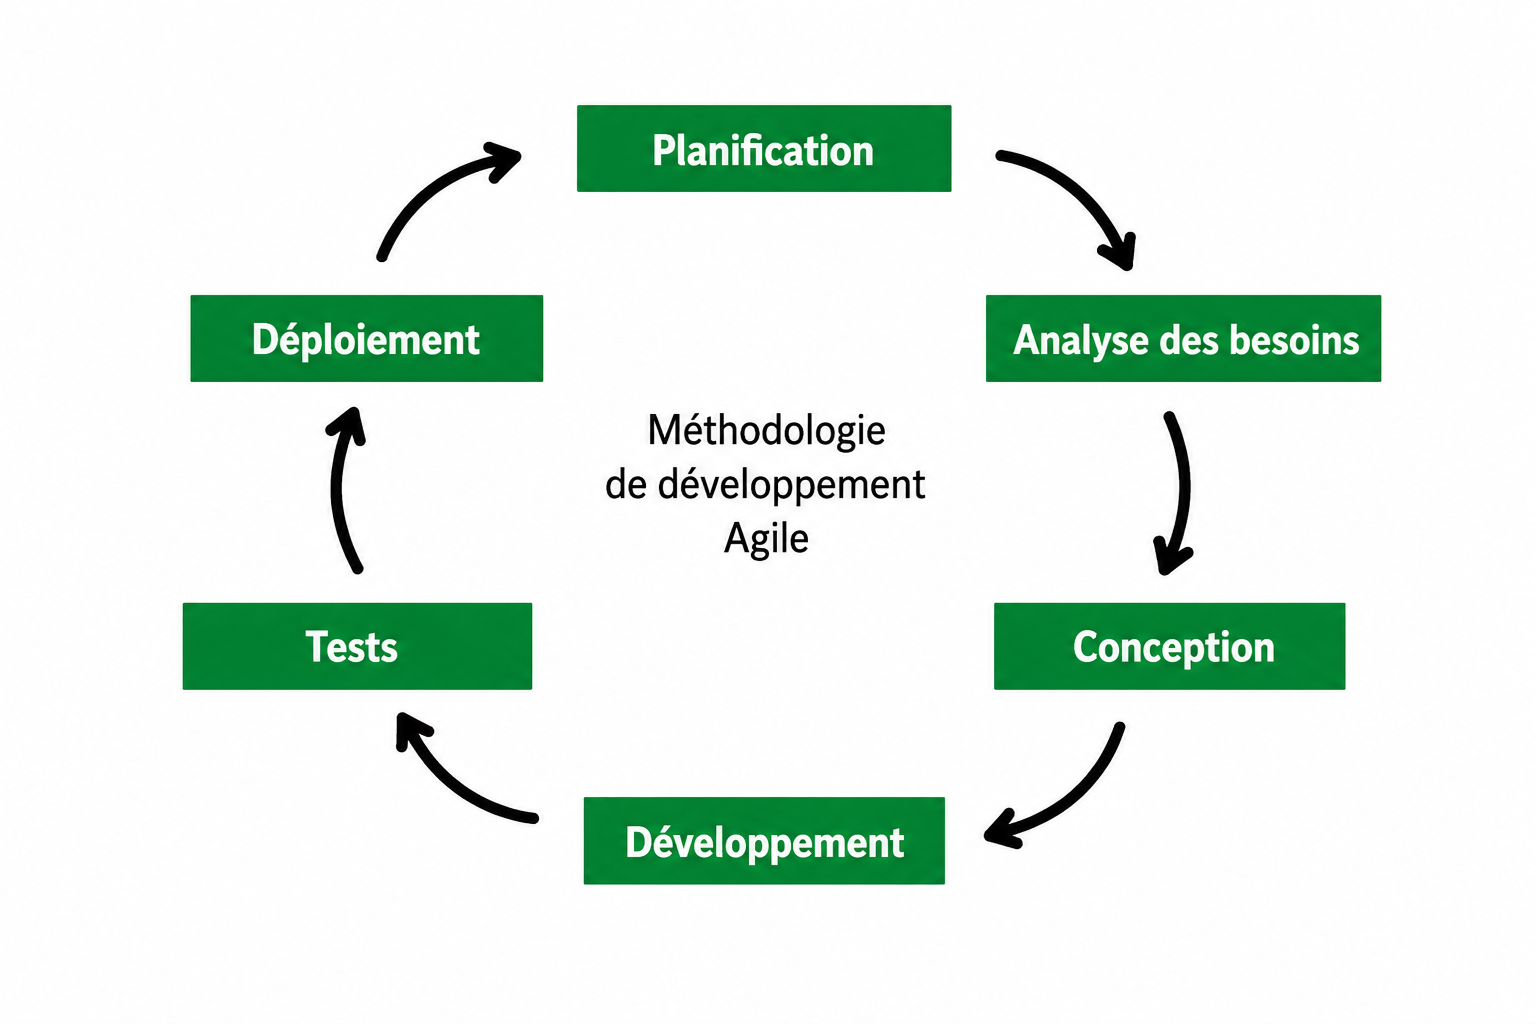
\includegraphics[width=0.75\textwidth]{img/methodologie.png}
    \caption{Cycle de développement Agile}
    \label{fig:agile_methodology}
\end{figure}

\par Comme illustré dans la Figure~\ref{fig:agile_methodology}, le développement s'est déroulé selon plusieurs phases successives : l'identification des besoins, la conception à l'aide d'UML et de l'architecture, la réalisation de l'application mobile sous Flutter, le développement du backend avec NestJS, les tests et la validation, puis le déploiement.

\par Cette organisation itérative a permis de développer progressivement les différentes fonctionnalités de l'application, de corriger rapidement les anomalies détectées et d'améliorer continuellement la solution.

\par Les principaux avantages de cette approche sont :

\begin{itemize}
    \item développement progressif de l'application ;
    \item adaptation aux évolutions des besoins ;
    \item validation régulière des fonctionnalités développées ;
    \item amélioration continue de la qualité de l'application.
\end{itemize}

\subsection{Framework SCRUM}

\par Afin d'organiser le développement, le framework SCRUM a été adopté \cite{scrum2020guide}. Les fonctionnalités de l'application ont été regroupées dans un \textit{Product Backlog} puis développées progressivement selon leur priorité.

\par Les premières itérations ont porté sur les fonctionnalités essentielles comme  l'authentification, la gestion des utilisateurs et la recherche de parkings. Les itérations suivantes ont permis d'intégrer la gestion des parkings privés, les sessions de stationnements, les paiements, les notifications ainsi que le système de recommandation basé sur l'IA.

\par À la fin de chaque itération, les fonctionnalités développées ont été testées et validées avant de procéder à la suivante. Cette organisation a permis de garantir une progression structurée du projet tout en assurant la qualité de la solution développée.

\section{Conclusion}

\par Dans ce chapitre, nous avons présenté le cadre général du TuniPark, la problématique étudiée, les solutions existantes ainsi que leurs principales limites. Nous avons ensuite proposé la solution retenue et présenté la méthodologie Agile ainsi que le framework SCRUM adoptés pour organiser le développement du projet.

\par Le chapitre suivant est consacré à l'analyse et à la spécification des besoins. Il présente les acteurs du système, les besoins fonctionnels et non fonctionnels ainsi que les principaux diagrammes UML utilisés pour la conception de l'application.